\section{Numerische Lineare Algebra, Lineare Gleichungssysteme}
\textbf{ZIEL}: Beantwortung folgender Fragen:
\begin{itemize}
\item{Gibt es Algorithmen, so dass große Abweichungen der berechneten Lösung (Lsg) zur tatsöchlichen nicht auftreten? 
  (``Es kommt darauf an'')}
\item{Kann man vorhersagen wann es zu großen Fehlern kommt, und wann nicht? (Ja)}
\end{itemize}

\begin{equation*}
  \left.
    \begin{aligned}
      \exists \widetilde{x} \neq 0: A\widetilde{x} = 0 & \Rightarrow  Ax = b \\
        & \Rightarrow A(x + \alpha \widetilde{x}) = b
%      \exists \widetilde{x} \neq 0: A\widetilde{x} = 0 \Rightarrow & Ax = b  \\
%      & A(x + \alpha \widetilde{x}) = b
%		\Fhat = \F \cup \F_d \hspace{0.5cm} \text{mit} \hspace{0.5cm} & \F && \text{normalisierte Gleitpunktzahlen}\\
%		 &\F_d && \text{denormalisierte Gleitpunktzahlen} 
    \end{aligned}
  \right\}
  \text{linear aber nicht eindeutig} %TODO christof: ich hab lösbar, aber nicht eindeutig stehen
\end{equation*}

\subsection{Grundlegendes}

\subsubsection{Matrix Norm}

Jede Norm über $\mathbb{K}^{m \times n}$ heißt Matrixnorm.
Matrixnormen lassen sich durch Vektornormen induzieren:
\begin{equation*}
\|A\|_p \coloneqq \underset{x \neq 0}{max} \frac{\|Ax\|_p}{\|x\|_p} = \underset{\|x\|_p = 1}{max}\|Ax\|_p
\end{equation*}

z.B.: $p \in \left\{1, 2, \infty \right\}$

Für induzierte Normen gilt:

\begin{itemize}
\item{$\|Ax\|_p \leq \|A\|_p \|x\|_p$}
\item{$\|A B\|_p \leq \|A\|_p \|B\|_p$}
\end{itemize}
Lässt sich einfach beweisen.

Im folgenden werden nur induzierte Normen verwendet.

\textbf{Satz:}
Sei $A \in \mathbb{K}^{m \times n}$. Dann gilt:
\begin{enumerate}[a)]
  \item{$\|A\|_1 = \underset{j = 1,..,n}{max} \sum\limits_{i=1}^{m}{\left|a_{ij}\right|}$ ( Spaltensummennorm )}
  \item{$\|A\|_{\infty} = \underset{j = 1,..,m}{max} \sum\limits_{i=1}^{n}{\left|a_{ij}\right|}$ ( Zeilensummennorm )}
  \item{$\|A\|_2 = \sqrt{\lambda_{max}\left(A^*A\right)}$}
\end{enumerate}
\textbf{Beweise:} a), b) durch einsetzen, c) benötigt Mittel aus linearen Algebra.

\subsubsection{$\left(Relative\right)$ Kondition einer Matrix}
Geg.: Sei $Ax = b$ (ungestörtes System), wobei
$A \in \mathbb{K}^{m \ times n}$ invertierbar und $b \in \mathbb{K}^n$ sei.  \\
Wie wirken sich Störungen $\Delta A$ und $\Delta b$ aus:  \\
\begin{align*}
  \left(A+\Delta A\right) \left(x+\Delta x\right)=b+\Delta b  \tag{gestörtes System}\\
  ? \quad \frac{\norm{\Delta x}}{\norm{x}} 
\end{align*}

Zunächst: Nur Störung von $b$ durch $\Delta b$, d.h. $A(x + \Delta x) = b + \Delta b$\\
$\Delta x = ?$
\begin{align*}
  A (x + \Delta x) &= b + \Delta b\\
  A \Delta x &= \Delta b\\
  \Delta x &= A^{-1} \Delta b\\
  \norm{\Delta x} &= \norm{ A^{-1} \Delta b } \leq \norm{A^{-1}} \norm{\Delta b}\\
  \norm{b} &= \norm{Ax} \leq \norm{A}\norm{b} \Rightarrow \frac{1}{\norm{x}} \leq \frac{\norm{A}}{\norm{b}} \\
  \Rightarrow \frac{\norm{\Delta x}}{\norm{x}} &\leq \norm{A}\norm{A^{-1}}\frac{\norm{\Delta b}}{\norm{b}} 
\end{align*}
\definition Sei $A$ invertierbar. $\kappa(A) := \norm{A}\norm{A^{-1}}$ heißt Konditionszahl von $A$ bzgl. $\norm{.}$.\\
\satz Sei $A$ invertierbar und $\Delta A$ sowie $\Delta b$ Störungen von $Ax=b$.
Dann gilt für hinreichend kleine $\Delta A$
\begin{align*}
  (A+\Delta A)(x + \Delta x) &= b + \Delta b\\
  \text{mit } \frac{\norm{\Delta x}}{\norm{x}} &\leq \frac{\kappa(A)}{1-\kappa(A)\frac{\norm{\Delta A}}{\norm{A}} } \left( \frac{\norm{\Delta A}}{\norm{A}} + \frac{\norm{\Delta b}}{\norm{b}} \right)
\end{align*}

TODO Fehlendes nachtragen
...

Berechnung von $\kappa_2\left(A\right)$
\begin{equation*}
  \begin{aligned}
    \kappa_2(A) = \|A\|_2 \|A^{-1}\|_2 = &\sqrt{\lambda_{max}\left(A^*A\right)} \cdot \frac{1}{\sqrt{\lambda_{min}\left(A^*A\right)}} \\
    = &\frac{\sigma_1\left(A\right)}{\sigma_n\left(A\right)}
  \end{aligned}
\end{equation*}
Für symmetrische und positiv definite $\frac{\sigma_1\left(A\right)}{\sigma_n\left(A\right)}$ Matrizen:
\begin{equation*}
  \kappa_2(A) = \frac{\lambda_{max}\left(A\right)}{\lambda_{min}\left(A\right)}
\end{equation*}

Bemerkung: Man beachte, dass in diesem Abschnitt die Konditionszahl einer Matrix $A$ definiert wurde und nicht die des Problems:
$Input\left(A,B\right) \rightarrow Output\left(A^{-1}b\right)$
Letzteres kann über den Ansatz in Abschnitt  berechnet werden und hängt eng mit $\kappa_A$ zusammen.

\textbf{Zeilenskalierung}
Bsp.: NUR DEMO!
\begin{equation*}
  \begin{aligned}
    \hspace{1cm} &Ax = \begin{pmatrix} 10^8 & 0 \\ 0 & 10^{-8} \end{pmatrix} x = \begin{pmatrix}b_1 \\ b_2\end{pmatrix} \\
    &\kappa_\infty\left(A\right) = 10^8 \cdot 10^8 = 10^{16}
  \end{aligned}
\end{equation*}
Vorkonditionierung durch Diagonalmatrix
\begin{equation*}
  D = \begin{pmatrix}10^{-8} & 0 \\ 0 & 10^8\end{pmatrix},
\end{equation*}
d.h. Löse statt Ax = b, dass dazu äquivalente System
\begin{equation*}
  \begin{aligned}
    &DAx = Db \\
    &\kappa_\infty\left(DA\right) = \kappa_\infty\left(I\right) = 1
	\end{aligned}	
\end{equation*}

Verbesserung der Konditionszahl bezgl. $\|.\|_\infty$ durch Zeilenskalierung.
Definiere: Diagonalmatrix:
\begin{equation*}
  D_z \left[ i,i \right] \coloneqq \left(\sum\limits_{j=1}^{n}{\left|a_{ij}\right|}\right)^{-1} %
\end{equation*}
Dann gilt:
\begin{equation*}
  \begin{aligned}
    &\sum\limits_{j=1}^{n}{\left|D_zA\left[i,j\right]\right|} = 1  \hspace{2cm} \text{für } 1, \ldots, n \\
    &\Rightarrow \|D_zA\|_\infty = 1
		\end{aligned}
\end{equation*}

\textbf{Satz:}
$\kappa_\infty\left(D_zA\right) \leq \kappa_\infty\left(DA\right)$ \hspace{2cm} $\forall$ regulären Diagonalmatrizen

\textbf{Beweis:}
Sei $A$ bereits äquilibriert, d.h.:
\begin{align*}
    &\sum\limits_{j=1}^{n}{\left|A\left[i,j\right]\right|} = 1 \hspace{2cm} \text{für } i = 1, \dots, n \\
	  &\Rightarrow \|A\|_\infty = 1 \\
	  &\Rightarrow \kappa_\infty\left(A\right) = \|A\|_\infty \|A^{-1}\|_\infty = \|A^{-1}\|_\infty
\end{align*}

Sei $D$ eine beliebige reguläre Diagonalmatrix
\begin{equation*}
\begin{aligned}
  \|DA\|_\infty = &\underset{1 \leq i \leq n}{max} \left\{\sum\limits_{j=1}^{n}{\left|d_ia_{ij}\right|}\right\} =
  \underset{1 \leq i \leq n}{max}\left\{\left|d_i\right|\sum\limits_{j=1}^{n}{\left|a_{ij}\right|}\right\} = \\
  &\underset{1 \leq i \leq n}{max}\left\{\left|d_i\right|\right\} = \|D\|_\infty = 
  \|\left(DA\right)^{-1}\|_\infty = \underset{x \neq 0}{max}\left\{\frac{\|A^{-1}D^{-1}x\|_\infty}{\|x\|_\infty}\right\} = \\
  &\underset{y \neq 0}{max}\left\{\frac{\|A^{-1}y\|_\infty}{\|Dy\|_\infty}\right\} \geq \underset{y \neq 0}{max}\left\{\frac{\|A^{-1}y\|_\infty}{\|D\|_\infty\|y\|_\infty}   \right\} \\
  &\Rightarrow \kappa_\infty\left(DA\right) = \|DA\|_\infty \|\left(DA\right)^{-1}\|_\infty \geq \\
  &\hcancel{$\|D\|_\infty$} \|A^{-1}\|_\infty \hcancel{$\|D\|_{\infty}^{-1}$} = \kappa_\infty\left(A\right)
\end{aligned}
\end{equation*}

\subsubsection{Residuum}
Sei $\widetilde
{x}$ eine Näherungslösung von GLS
\begin{equation*}
Ax=b
\end{equation*}
Dann bezeichnet man
\begin{equation*}
r \coloneqq r_{\widetilde{x}} \coloneqq A\widetilde{x} - b
\end{equation*}

als Residuum.
\textbf{ACHTUNG:}
\begin{itemize}
  \item{Residuum ist nicht der Fehler von $\widetilde{x}$}
	\item{Für die exakte Lösung $x$ gilt:}
\end{itemize}
\begin{equation*}
r_x = Ax - b = 0
\end{equation*}

Frage: Ist $r_{\widetilde{x}}$ ein guter Indikator dafür, wie genau $\widetilde{x}$ ist?
Antw.: Nein, außer Matrix ist gut Knoditioniert!

\textbf{Satz:}
Sei $a \in \mathbb{K}^{n \times n}$ invertierbar und $\widetilde{x}$ Näherungslösung von
\begin{equation*}
\begin{aligned}
Ax = b \hspace{2cm} b \neq 0
\end{aligned}
\end{equation*}
Dann gilt:
\begin{equation*}
\frac{\|x - \widetilde{x}\|}{\|x\|} \leq \kappa\left(A\right) \frac{\|r\|}{\|b\|}
\end{equation*}
\textbf{Beweis:}
\begin{equation*}
\begin{aligned}
r &= A\widetilde{x} - b = A\widetilde{x} - Ax = A\left(\widetilde{x} - x\right) \\
&\Rightarrow \widetilde{x} - x = A^{-1}r \\
&\|\widetilde{x} - x\| = \|A^{-1}r\| \leq \|A^{-1}\|\|r\| \\
&\|b\| = \|Ax\| \leq \|A\|\|x\| \\
&\frac{1}{\|x\|} \leq \frac{\|A\|}{\|b\|}
\end{aligned}
\end{equation*}

\begin{figure}[htbp]
  \centering
  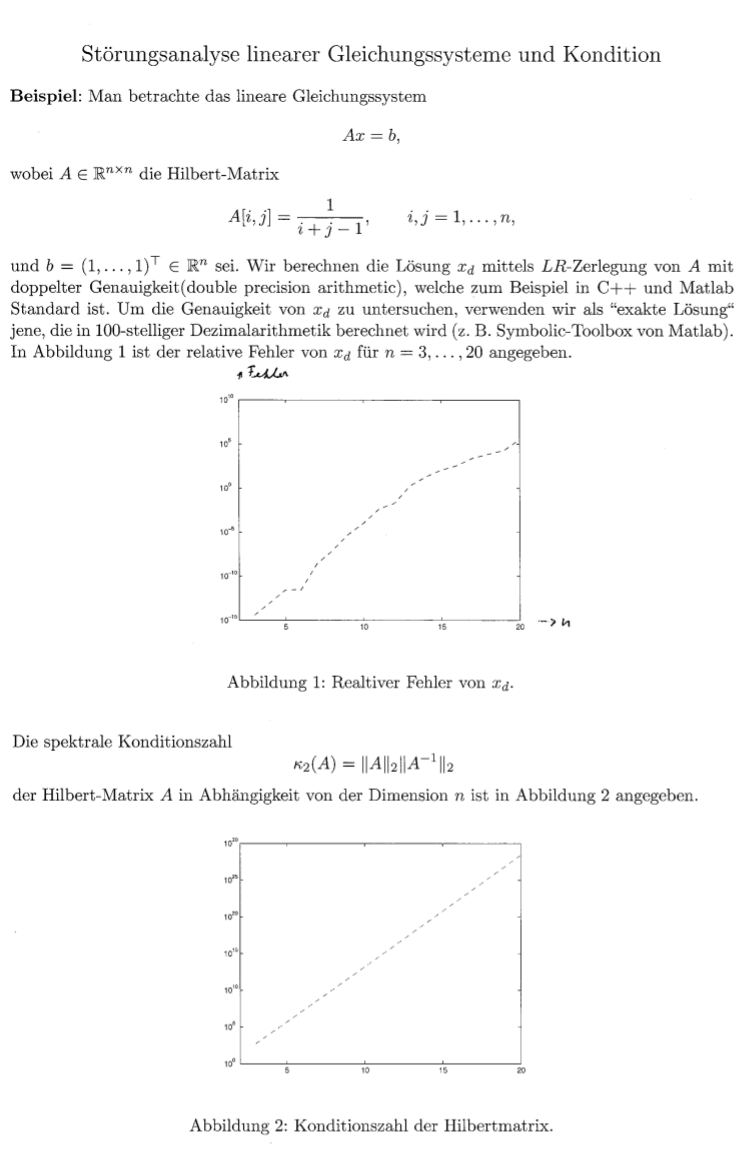
\includegraphics[width=0.9\textwidth]{figures/stoerungsanalyse_lin_glgns.png}
\end{figure}

\subsection{Direkte Lösung von Linearen Gleichungssystemen (in n - Schritten exakte Lsg)}
\subsubsection{Gauß - Algorithmus und LR - Zerlegung}
Zunächst: Voraussetzung das Gauß - Algorithmus ohne Zeilen verauschen druchführbar sei:

\begin{equation*}
  \begin{aligned}
    Ax = b \\
    &a_{11}^{\left(1\right)}x_1 + \ldots + a_{1n}^{\left(1\right)}x_n = b_1^{\left(1\right)}  \\
    &\vdots                               \vdots                     = \vdots  \\
    &a_{n1}^{(1)}x_1 + \ldots + a_{nn}^{(1)}x_n = b_n^{(1)}  \\
  \end{aligned}
\end{equation*}

1.Schritt: Subtrahiere das $\left(\frac{a_{i1}}{a_{11}}\right) =: L_{i1}$ - fache der 1. Zeile
von der i-ten Zeile, i = 2, ..., n.
\begin{align*}
    a_{11}^{(1)}x_1 + \ldots + a_{1n}^{(1)}x_n = b_1^{(1)}  \\
		\vdots                    +a_{22}^{(2)}x_2 \ldots + a_{1n}^{(2)}x_n = b_2^{(2)}  \\
    \vdots                               \vdots                     = \vdots  \\
    \ldots  + a_{2n}^{(2)}x_2 + a_{nn}^{(2)}x_n = b_n^{(2)} \\
\end{align*}
\begin{align*}
    A^{(2)} = L_1A^{(1)}, \text{wobei dieses bleibt gleich} \\
\end{align*}
\begin{align*}
    L_1 = \begin{pmatrix} 1 & \ldots &        &  \\ 
		                -L_{21} & 1      & 0      &  \\
					          \vdots	& 0      & \ddots &  \\
										-L_{n1} & \ldots &        & 1
					\end{pmatrix}
\end{align*}
\begin{align*}
		s. Schritt: A^{\left(s\right)} = L_{s-1}A^{\left(s-1\right)} \\
\end{align*}
\begin{align*}
		A_s = \begin{pmatrix}
		      a_{11}^{\left(1\right)} & a_{12}^{\left(1\right)} & \ldots & \ldots & a_{1n}^{\left(1\right)} \\
					\vdots                  & a_{22}^{\left(2\right)} & \ldots & \ldots & a_{2n}^{\left(2\right)} \\
					\vdots                  & \ddots                  & \ldots & \ldots & \vdots                  \\
					                        &                         & a_{ss}^{\left(s\right)} & \ldots  & a_{sn}^{\left(s\right)} \\
																	&                         & a_{ns}^{\left(s\right)} & \ldots  & a_{nn}^{\left(s\right)}
		      \end{pmatrix}
					b = \begin{pmatrix}b_1^{\left(1\right)} \\ b_2^{\left(2\right)} \\ \vdots \\ b_s^{\left(s\right)} \\ b_n^{\left(s\right)}\end{pmatrix}\\
\end{align*}
\begin{align*}
		L_s = \begin{pmatrix}
		      1 &   &        &            &        &        & \\
					  & 1 &        &            &        &        & \\
						&   & \ddots &            &        &        & \\
						&   &        & 1          &        &        & \\
						&   &        & -L_{s+1,s} & \ddots &        & \\
						&   &        & \vdots     &        & \ddots & \\
						&   &        & -L_{ns}    &        &        & 1
		      \end{pmatrix}
\end{align*}
\begin{align*}
  L_{i,s} = \frac{a_{i,s}^{(s)}}{a_{s,s}^{(s)}} \text{für } i = s + 1, \ldots, n
\end{align*}

Schritt n-1: $A^{\left(n\right)} = L_{n-1}A^{n-1}$
Rechte obere
$\Delta$-Matrix

D.h.: 
\begin{equation*}
  \begin{aligned}
A = A^{(1)} \rightarrow A^{(2)} = L_1A^{(1)} \rightarrow A^{(3)} = L_2A^{(2)} \ldots \rightarrow A^{(n)} = L_{n-1}A^{(n-1)} \\
A^{(3)} = L_2L_1A^{(1)}
  \end{aligned}
\end{equation*}
bzw.
\begin{equation*}
  \begin{aligned}
    R = A^{(n)} = L_{n-1} \ldots L_1 A  \\
		(L_{n-1}, \ldots, L_1)^{-1}R = A  \\
		\underbrace{(L_1^{-1} \cdot \ldots \cdot L_{n-1}^{-1})}{=:L}R = A  \\
%		=: L  und  \\
		L = \begin{pmatrix}
		    1      &        &        &  \\
				L_{21} & \ddots & 0      &  \\
				\vdots &        & \ddots &  \\
				L_{n1} & \ldots & L_{n\left(n-1\right)} & 1
		    \end{pmatrix}
	\end{aligned}
\end{equation*}

\textbf{Beweis:}
Lässt sich über nachrechnen leicht überprüfen

\textbf{LR = A} % Todo: sollte in einer Box sein!
Algorithmus (Gauß a. - ohne Zeilen vertauschen)
\begin{equation*}
  for s = 1, .., n-1  \\
	  for i = s+1, ..., n  \\
		  L_{is} = \frac{a_{is}}{a_{ss}^{\left(s\right)}}  \\
			b_i^{\left(s+1\right)} = b_i{\left(s\right)} - L_{is}b_s^{\left(s\right)}
			[a_{i, s+1}^{(s+1)} \ldots a_{i,n}^{(s+1)}] = [a_{i, s+1}^{(s)} \ldots a_{i,n}^{(s)}] - L_{i,s}[a_{s,s+1}^{(s)} \ldots a_{s,n}^{(s)}]
		end
	end
\end{equation*}
%
\textbf{Satz:}
Für den Gauß - Algorithmus sind $\frac{2}{3}n^3 + \mathcal O(n^2)$ Arithmetische Operationen erforderlich.

\textbf{Beweis:}
Schritt s: (s = 1, .., n-1)
\begin{equation*}
  \begin{aligned}
	  : n-s [s+1, s+2, \ldots, s+n - s] \\
		\cdot n-s + (n-s)(n-s) = n^2 - 2ns +s^2 \\
		- n-s + (n-s)(n-s) \\
		\hline
		\underbrace{2 \cdot \sum\limits_{s=1}^{n-1}{s^2}}{2 \frac{(n-1)n(2n-1)}{6}}+\underbrace{\sum\limits_{s=1}^{n-1}{s}}_{3\frac{(n-1)n}{2}}
	\end{aligned}
\end{equation*}

TODO nachschauen ob sicher nichts fehlt\\

Zeitaufwand für Gauß-Verfahren Intel Core i7, 3GHz $\approx 100$GFlops:\\
\begin{tabular}{c | r l}
  $n = 10^4$ & $6,6$ &s\\
  $n = 10^5$ & $1,85$ &h\\
  $n = 10^6$ & $77$ &Tage
\end{tabular}\\
Gauß-Verfahren mit Zeilenvertauschung (Spaltenpivotisierung)\\
Zu Beginn des Schrittes s sucht man das größte Element von $[a_{ss}^{(s)}\ldots a_{ns}^{(s)}]^T$
und vertausche Zeile s mit derjenigen Zeile, die das größte Element des obigen Vektors hat.
Dies ist notwendig:
\begin{itemize}
  \item damit GV i.A. durchführbar ist,
  \item wegen numerischer Stabilität (siehe später)
\end{itemize}
\satz Sei $A \in \mathbb{K}^{n \times n}$ regulär, dann existiert eine Permutationsmatrix $P$,
so dass $PA = LR$ ist, wobie $L$ linke und $R$ rechte Dreiecksmatrix ist.\\
\beweis Findet man in jedem Numerik-Lehrbuch\\
\matlab{lu(A)}\\

Die Lösung $Ax=b$ mittels LR-Zerlegung:\\
$Ax = b \Leftrightarrow PAx = Pb \Leftrightarrow L\underbrace{Rx}_{y} = Pb \Leftrightarrow [Ly = Pb \text{ und } Rx = y]$
\begin{enumerate}
  \item LR-Zerlegung von A: Aufwand $\frac{2}{3} n^3 + \LandauO(n^2)$
  \item Löse $Ly = Pb$ (``Vorwärtseinsetzen''): $n^2$
  \item Löse $Rx = y$ (``Rückwärtseinsetzen''): $n^2$
\end{enumerate}
Gesamtaufwand: $\frac{2}{3} n^3 + \frac{3}{2} n^2 + \LandauO(n) \qquad (A \in \mathbb{R}^{n \times n})$\\
Anteil von Vorwärst- und Rückwärtseinsetzen an den Gesamtkosten $\approx \frac{3}{n}$.\\
Bei $n=100 \quad 3\%$; bei $n=1000 \quad 0,3\%$

Bsp: GV ohne Spaltenpivotisierung
\begin{align*}
  A = \begin{pmatrix}
    10^{-20} & 1\\
    1        & 1
  \end{pmatrix}
  ,\quad b = \begin{pmatrix} 3 \\ 3 \end{pmatrix}
\end{align*}
$Ax = b$ Matrix $A$ ist gut konditioniert: $\kappa_2(A) = 2,6$\\
$\Rightarrow x = \begin{pmatrix} 0 \\ 3 \end{pmatrix}$ [``cond(A,2)'', Eigenvalue $A^* A$ (größerer)]\\
GV mit $eps = 10^{-16}$\\
$rd(1-10^{20}) = -10^{20}$
\begin{align*}
  \hat{R} = \begin{pmatrix}
    10^{-20} & 1 \\
    0 & -10^{20}
  \end{pmatrix} && \hat{L} = \begin{pmatrix}
    1 & 0 \\
    10^{20} & 1
  \end{pmatrix}\\
  \hat{L} y = b: & \begin{pmatrix} 1 & 0 \\ 10^{20} & 1 \end{pmatrix} \begin{pmatrix} y_1 \\ y_2 \end{pmatrix} =
  \begin{pmatrix} 3 \\ 3 \end{pmatrix} \Rightarrow \begin{pmatrix} y_1 \\ y_2 \end{pmatrix} = \begin{pmatrix}
    3 \\ \underbrace{3 - 3\cdot 10^{20}}_{-3 \cdot 10^{20}}
  \end{pmatrix}\\
  \hat{R} x = y: & \begin{pmatrix} 10^{-20} & 1 \\ 0 & -10^{20} \end{pmatrix} \begin{pmatrix} x_1 \\ x_2 \end{pmatrix} =
  \begin{pmatrix} 3 \\ -3 \cdot 10^{20} \end{pmatrix} \Rightarrow x_2 = 3\\
  10^{-20}x_1 + 3 = 3 \Rightarrow x_1 = 0\\
  \text{Aber: } & \hat{L}\hat{R} = \begin{pmatrix} 10^{-20} & 1 \\ 1 & 0 \end{pmatrix} \\
  & \hat{L}\hat{R} \begin{pmatrix} \hat{x}_1 \\ \hat{x}_2 \end{pmatrix} = \begin{pmatrix} 3 \\ 3 \end{pmatrix} \\
  & \Rightarrow \hat{x}_1 = \hat{x}_2 = 3
\end{align*}
\begin{align*}
  \frac{\norm{\hat{x}-x}_{\infty}}{\norm{x}_\infty} = 100\%
\end{align*}
% subsubsubsection
\para{Fehleranalyse des Gauß-Verfahrens}
Einfluss von Rundungsfehlern?\\

\satz Sei $A \in \mathbb{C}^{n \times n}$ regulär und $b \in \mathbb{C}^n$. Seien $\hat{L}$ und $\hat{R}$ die mittels GV
berechneten Faktoeren der LR-Zerlegung von $A$ und $\hat{x}$ die berechnete Lösung für $Ax = b$, wobei mit
Maschinengenauigkeit $eps$ gerechnete wurde. Dann gilt:
\begin{align*}
  \frac{\norm{\hat{x}-x}_\infty}{\norm{x}_\infty} \leq \kappa(A) 3n^2 eps \norm{\hat{R}} + \LandauO(eps^2) \tag{*}
\end{align*}
\beweis Siehe Demmel (1999), Abs. 2.4.\\
Diskussion von (*):
\begin{enumerate}
  \item Der relative Fehler von $\hat{x}$ ist meist viel kleiner als in (*), $n^2$ wird nur im worst case angenommen
  \item Was weiß man über $\norm{\hat{R}}$?
    \begin{enumerate}[i]
      \item $\norm{\hat{R}}$ kann sehr groß werden, z.B. $2^{n-1}$
      \item Matrizen für die $\norm{\hat{R}}$ groß ist, sind sehr ``unwahrscheinlich'', was
        \begin{itemize}
          \item Experimente mit Zufallsmatrizen
          \item Anwendungsbeispiele in der Praxis
        \end{itemize}
        gezeigt haben.
    \end{enumerate}
\end{enumerate}

\begin{figure}[htbp]
  \centering
  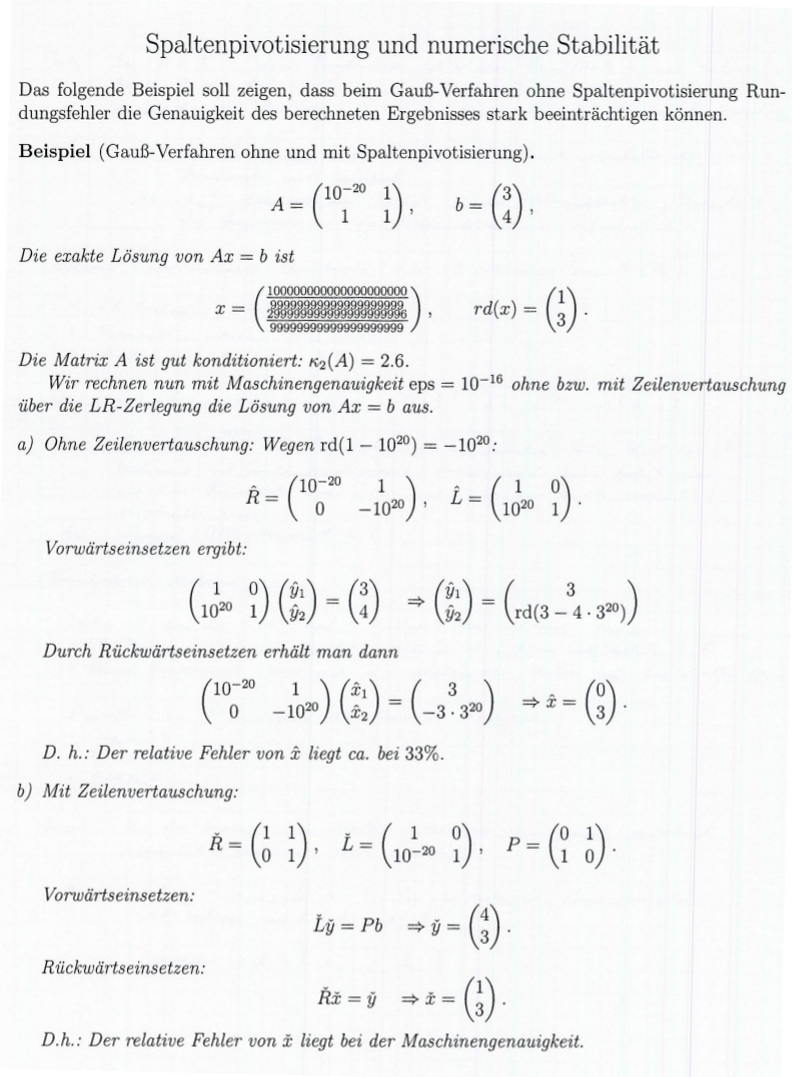
\includegraphics[width=\textwidth]{figures/spaltenpivotisierung.png}
\end{figure}
% subsubsubsection
\para{LR-Zerlegung für Bandmatrizen}
\definition Die Matrix
\begin{align*}
  A = \begin{pmatrix}
    a_{1,1} & \cdots & a_{1,p+1} & 0         & \cdots & 0\\
    \vdots  & \ddots &           & a_{2,p+2} & & \\
    a_{q+1,1} &      & \ddots    &           & \ddots & \\
    0       & a_{q+2,2} &        & \ddots    & & a_{n-p,n} \\
    \vdots  & \ddots & \ddots    &           & \ddots & \vdots \\
    0       & \cdots & 0         & a_{n,n-q} & \cdots & a_{n,n} \\
  \end{pmatrix}
\end{align*}
beziechnet man als Bandmatrix mit oberer Bandbreite $p$ und unterer Bandbreite $q$.
\begin{figure}[htbp]
  \centering
  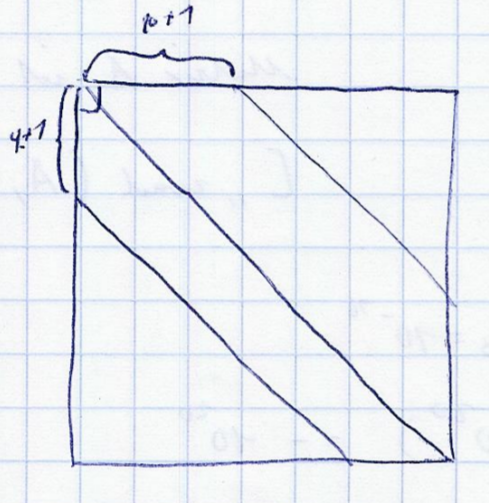
\includegraphics[width=0.3\textwidth]{figures/bandmatrix.png}
  \caption{Bandmatrix}
\end{figure}
\satz Sei $A \in \mathbb{R}^{n \times n}$ eine Bandmatrix mit oberer Bandbreite $p$
und unterer Bandbreite $q$. Die LR-Zerlegung sei ohne Zeilenvertauschung durchführbar.
Dann hat $L$ untere Bandbreite $q$ und $R$ obere Bandbreite $p$.\\
\beweis
\begin{itemize}
  \item Zur Bestimmung von $R$ werden die Elemente oberhabl der Bandbreite nicht geändert.
  \item $l_{ij}$ beschreibt den Faktor für die Zeilensubtraktion. Unterhalb der Bandbreite
    sind keine Zeilesubtraktionen erforderlich.
\end{itemize}
Aufwand (arithmetische Opertionen) der LR-Zerlegung von $A \in \rnxn$
\begin{enumerate}
  \item LR-Zerlegung: $\approx 2 n pq$
  \item Vorwärtseinsetzen: $\approx 2 nq$
  \item Rückwärtseinsetzen: $\approx 2 np$
\end{enumerate}
Gasmt: $2n (pq + q + p)$, d.h. $\LandauO(n)$ für $n \gg \max\{ p, q \}$\\
\satz Sei $A \in \rnxn$ eine Bandmatrix, wie im letzten Satz. Wird die LR-Zerlegung
mit Spaltenpivotisierung durchgeführt, dann hat $R$ eine max. obere Bandbreite von
$p + q$ und $L$ hat pro Spalte maximal $q$ Nichtnulleinträge.\\
\beweis Demmel (1999), Abschnitt 2.7.3
\para{Dünnbesetzte Matrizen}
Treten z.B. bei der FEM auf. \matlab{sparse} Matrixklasse
\begin{itemize}
  \item LR-Zerlegung von dünnbesetzten Matrizen $\Rightarrow$ i.A. zu vollbesetzten $L$, $R$
  \item Durch Umsortierung lässt sich eine dünnbesetzte Matrix auf Bandstruktur bringen
\end{itemize}
Algorithmen zur LR-Zerlegung dünnbesetzter Matrizen:
\begin{itemize}
  \item Super LU
  \item UMFPACK
  \item PARDISO
\end{itemize}
Regel: Nie die Inverse einer Matrix berechnen, wenn nicht unbedingt erforderlich (numerisch sehr instabil)\\
Wenn $Ax_k = b_k$ für $k = 1,\ldots,m$ zu lösen ist, dann berechne LR-Zerlegung von A und nicht $A^{-1}$.\\
\matlab{$A\backslash[b_1,\ldots,b_m]$}

\subsubsection{Cholesky-Zerlegung}
\definition Eine Matrix $A$ heißt symmetrisch / hermitesch positiv definit (s.p.d),
falls $A^* = A$ und $x^*Ax > 0\,\forall x \neq 0$.\\
Treten häufig auf, z.B.: FEM, Ausgleichsrechnung, Optimierung\\
\satz Sei $A$ s.p.d., dann gilt:
\begin{enumerate}[a]
  \item $a_{ii} > 0$
  \item alle Eigenwerte von $A$ sind positiv (hinreichende Bedingung)
  \item $\kappa_2(A) = \frac{\lambda_{max}(A)}{\lambda_{min}(A)}$
\end{enumerate}
\satz Sei $A \in \rnxn$ s.p.d., dann existiert eine untere (linke) Dreiecksmatrix $L$
mit $A = LL^*$ (Cholesky Zerlegung)\\
Algorithmus:\\
\begin{flalign*}
  & \texttt{for } k = 1:n\\
  & \quad l_{kk} = \left( a_{kk} - \sum^{k-1}_{j=1} \abs{l_{kj}}^2 \right)^{\frac{1}{2}}\\
  & \quad \texttt{for } i=k+1:n\\
  & \qquad l_{ik} = \frac{a_{ik} - \sum^{k-1}_{j=1} l_{ij} \bar{l}_{kj}}{l_{kk}} \\
  & \quad \texttt{end}\\
  & \texttt{end}
\end{flalign*}
\beweis Siehe Lehrbuch Numerik\\
Eigenschaften:\\
\begin{itemize}
  \item Aufwand $\frac{1}{3} n^3 + \LandauO(n^2)$ Flops für $A \in \rnxn$
  \item Numerisch stabil ($Ax=b$): $\frac{\norm{\hat{x}-x}_\infty}{\norm{x}_\infty} \leq \kappa_\infty(A) 3n^2 eps + \LandauO(eps)$
\end{itemize}
d.h. ist $A$ gut konditioniert, dann kann der Fehler nicht ``explodieren''.\\
Ist Matrix nicht s.p.d., dann kommt bei obigem Algorithmus NaN heraus.\\
\matlab{chol(A)}

\subsubsection{QR-Zerlegung}
\definition Eine Matrix $A \in \rmxn$ mit $m \geq n$ sei gegeben. Die Faktorisierung $A = QR$ (siehe Abbildung~\ref{fig:qr}) wobei $Q$
eine unitäre Matrix ($Q^*Q=I$) und $R$ eine verallgemeinerte obere Dreiecksmatrix sei, 
d.h. $r_{ij} = 0$ für $i > j$ heißt QR-Zerlegung von $A$.
\begin{figure}
  \centering
  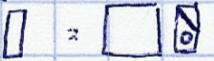
\includegraphics[width=0.1\textwidth]{figures/qr.png}
  \caption{Matrixformen der QR-Zerlegung}
  \label{fig:qr}
\end{figure}
\definition $Q \in \raxb{m}{m}$ heißt unitär, wenn $Q^*Q=QQ^*=I$\\
Es gilt: $Q^*Q=I \Leftrightarrow$ Die Spalten bzw. Zeilen von $Q$ sind orthonormal bzgl. $\inner{.}{.}_2$.\\
Eigenschaften unitärer Matrizen:
\begin{itemize}
  \item $\norm{Qx}_2^2 = (Qx)^*Qx = x^*\underbrace{Q^*Q}_{I}x = x^*x = \norm{x}_2^2 \Rightarrow$ Längenerhaltung, Drehungen
  \item Es lässt sich einfach zeigen: $\norm{QA}_2 = \norm{AQ}_2 = \norm{A}_2$
  \item $\kappa_2(Q) = \sqrt{\frac{\lambda_{max}(Q^*Q)}{\lambda_{min}(Q^*Q)}} = 1$
\end{itemize}
\satz Sei $A \in \rmxn$ Dann existiert eine QR-Zerlegung der Form 
\begin{align*}
  A=QR=\begin{pmatrix} Q_1 & Q_2 \end{pmatrix} \begin{pmatrix} R_1 \\ 0 \end{pmatrix} = Q_1 R_1
\end{align*}
\beweis Siehe Lehrbuch Numerik\\
Eigenschaften und Einsatz der QR-Zerlegung:
\begin{itemize}
  \item Sei $A \in \rnxn$ regulär. Durch die QR-Zerlegung wird die Kondition von $Ax=b$ nicht verschlechtert, denn:
    \begin{itemize}
      \item Man löst: $Rx = Q^*b \quad (Ax = b \Leftrightarrow QRx = b \Leftrightarrow Rx = Q^*b)$
      \item Man kann zeigen $\kappa_2(A) = \kappa_2(QR) = \kappa_2(R)$
    \end{itemize}
  \item QR-Zerlegung ist numerisch stabiler als LR-Zerlegung \begin{align*}
      \frac{\norm{\hat{x} - x}}{\norm{x}} \leq c\,eps\,\kappa_\infty(A)n^2 + \LandauO(eps^2)
    \end{align*}
  \item QR-Zerlegung ist doppelt so teuer wie LR-Zerlegung
  \item Einsatz: Ausgleichsrechnung
\end{itemize}
Methoden zur QR-Zerlegung:
\begin{itemize}
  \item Householder-Verfahren
  \item Given-Verfahren
  \item Gram-Schmidt-Verfahren
\end{itemize}
\matlab{qr(A)}

\subsection{Lineare Ausgleichsrechnung}
Bsp.: Es seien $(t_i, y_i),\,i=1,\ldots,m$ gegeben.\\
Gesucht: 
\begin{align*}
  y(t) := \sum^{n}_{j=1} x_j \phi_j(t) \tag{ + }
\end{align*}
wobei
\begin{itemize}
  \item $\phi_i$ gegebene Funktionen $j=1,\ldots,n$
  \item $y(t_i) \approx y_i \qquad i=1,\ldots,m$
  \item $m > n$
\end{itemize}
\begin{figure}
  \centering
  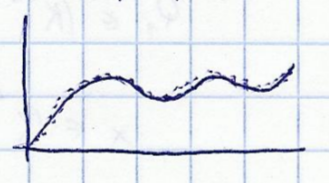
\includegraphics[width=0.4\textwidth]{figures/lineare_ausgleichsrechnung.png}
  \caption{Lineare Ausgleichsrechnung}
\end{figure}
D.h. mehr Messdaten als Unbekannte $(x_1,\ldots,x_n)$\\
Setze Messdaten in (+) ein:
\begin{align*}
  y_i = \sum^{n}_{j=1} x_j \phi_j(t_i) \qquad i=1,\ldots,m\\
  Ax=b \text{ überbestimmtes Gleichungssystem } \Rightarrow \text{ i.A. nicht lösbar}\\
  A[i,j] = \phi_j(t_i), \quad b_i = y_i
\end{align*}
\definition Sei $A \in \rmxn$ und $b \in \ra{m}$. Das lineare Ausgleichsproblem (LAP) besteht darin ein $x \in \ra{n}$ mit
\begin{align*}
  \norm{Ax-b}_2 = \underset{y \in \ra{n}}{\min} \norm{Ay - b}_2
\end{align*}
\satz Sei $A \in \rmxn$ und $b \in \ra{m}$. Dann gilt:
\begin{enumerate}[a)]
  \item LAP besitzt mindestens eine Lösung
  \item $x \in \ra{n}$ ist Lösung von LAP $\Leftrightarrow$ $x$ Lösung der Gaußschen Normalengleichung (GNG)
  \item Für $m \geq n$ und $\mathrm{Rang}(A) = n$ besitzt LAP genau eine Lösung

\end{enumerate}
\beweis
\begin{enumerate}[a)]
  \item siehe Numerik-Lehrbuch
  \item{Das lineare Ausgleichsproblem \begin{align*}
    \norm{Ax-b}_2 = \underset{y \in \ra{n}}{\min} \norm{Ay - b}_2\\
    \norm{a_1 x_1 + \ldots + a_n x_n - b} = \underset{y \in \ra{n}}{\min} \norm{a_1 y_1 + \ldots + a_n x_n - b}
    \end{align*} lässt sich als BA-Aufgabe von $b$ bzgl. $\norm{.}$ im Raum $\mathrm{span}\{a_1, \ldots, a_n\}$ interpretieren,
    wobei $Ax$ die BA ist.
    \begin{figure}
      \centering
      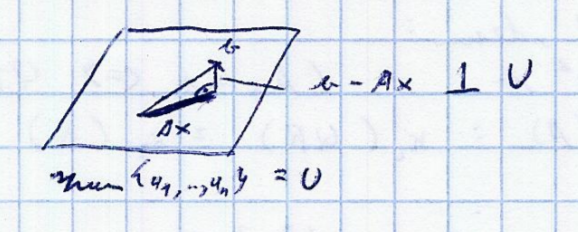
\includegraphics[width=0.4\textwidth]{figures/ausgleichsrechnung_ba.png}
      \caption{Bestapproximation}
    \end{figure}
    \begin{align*}
      \inner{b - Ax}{u}_2 &= 0 \qquad & \forall u \in \mathrm{span}\{a_1,\ldots, a_n\}\\
      &\Updownarrow\\
      \inner{b - Ax}{a_j}_2 &= 0 & \text{für } j=1,\ldots,n\\
      &\Updownarrow\\
      \inner{Ax}{a_j}_2 &= \inner{b}{a_j} \qquad & \text{\ditto}\\
      &\Updownarrow\\
      (a_j)^* Ax &= (a_j)^* \qquad & \text{\ditto} \Leftrightarrow A^*Ax = A^* b \tag{GNG}
    \end{align*}}
  \item Eindeutige Lösbarkeit folgt aufgrund der positiven Definitheit von $A^*A$, siehe Numerik-Lehrbuch.
\end{enumerate}
Im Folgenden setzen wir c) des letzten Satzes voraus.

Lange Zeit wurde GNG verwendet um LAP zu lösen (mittels Cholesky-Zerlegung).
Allerdings ist GNG oft sehr schlecht konditioniert.\\
\satz Sei $A \in \rmxn,\,m \geq n$ und $\mathrm{rg}(A) = n$. Sei $A = QR = \mat{Q_1 & Q_2} \mat{R_1 \\ 0}$.
$Q_1 \in \rmxn,\, R_1 \in \rnxn$ eine QR-Zerlegung. Dann gilt:
\begin{align*}
  x \in \ra{n} \text{ ist Lösung von LAP } \Leftrightarrow R_1 x = Q_1^* b
\end{align*}
\beweis Es gilt: $\norm{Qx}_2 = \norm{x}_2,\quad Q^*Q = I = QQ^*$\\
\begin{align*}
  \norm{Ax - b}_2^2 &= \norm{QRx - b}_2^2 \\
  &= \norm{QRx - QQ^*b}_2^2 \\
  &= \norm{Q(Rx - Q^*b)}_2^2 \\
  &= \norm{Rx - Q^*b}_2^2 \\ 
  &= \norm{\mat{R_1 \\ 0}x - \mat{Q_1 & Q_2}^* b}_2^2\\
  &= \norm{\mat{R_1x & -Q_1^*b \\ 0 & -Q_2^*b}}_2^2 \\
  &= \norm{R_1 x - Q_1^*b}_2^2 + \norm{Q_2^* b}_2^2
\end{align*}
$R_1$ ist regulär weil $\mathrm{rg}(A) = n$. Damit erhält man für $x \in \ra{n}$:
\begin{align*}
  \norm{Ax -b}_2^2 \text{ ist minimal } \Leftrightarrow \norm{R_1x - Q_1^*b}_2^2 = 0 \Leftrightarrow R_1x = Q_1^*b
\end{align*}
QR-Zerlegung ist der GNG vorzuziehen, weil sie numerisch stabiler ist und der Aufwand ca. gleich ist.

\subsubsection{Singulärwertzerlegung (SVD)}
SVD ist ein bedeutendes theoretisches und praktisches Hilfsmittel.\\
\satz Sei $A \in \mathbb{K}^{m \times n}$, $\mathrm{rg}(A) = r$\\
\begin{enumerate}
  \item{Es existieren reelle Werte $\sigma_1 \geq \sigma_2 \geq \ldots \geq \sigma_r > 0$, sowie
      unitäre Matrizen $U \in \mathbb{K}^{m \times m}, \, V \in mathbb{K}^{n \times m}$, so dass
      \begin{align*}
        A = U \Sigma V^* \tag{SVD}
      \end{align*}
      \begin{figure}[htbp]
        \centering
        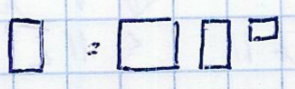
\includegraphics[width=0.2\textwidth]{figures/svd.png}
        \caption{Matrixformen SVD}
      \end{figure}
      wobei
      \begin{align*}
        \Sigma = \begin{pmatrix}
          \sigma_1 &        &          & 0 \\
                   & \ddots &          &   \\
                   &        & \sigma_r &   \\
          0        &        &          & 0
        \end{pmatrix}
      \end{align*}}
  \item{Die (positiven) Diagonalelemente von $\Sigma$ bezeichnet man als Singulärwerte von $A$.
      Die Singulärwerte stimmen mit den Eigenwerten von $A^*A$ und $AA^*$ überein und sind eindeutig
      bestimmt. Wurzeln der Eigenwerte von U und V sind nicht eindeutig.}
    \item Für reguläres $A \in \mathbb{K}^{n \times n}$ gilt: $\kappa_2(A) = \frac{\sigma_1(A)}{\sigma_n(A)}$
\end{enumerate}
\matlab{svd(A)}\\
SVD lässt sich als Eigenwertproblem definieren.\\
Sei $A = U \Sigma V^*$ eine SVD von A:
\begin{align*}
  A &=\mat{a_1 & \ldots & a_n} \begin{pmatrix}
          \sigma_1 &        &          & 0 \\
                   & \ddots &          &   \\
                   &        & \sigma_r &   \\
          0        &        &          & 0
        \end{pmatrix} \begin{pmatrix}
          v_1^* \\ \vdots \\ v_n^* 
        \end{pmatrix}
        = \mat{a_1 & \ldots & a_n} \mat{\sigma_1 v_1^* \\ \vdots \\ \sigma_r v_r^* \\ 0} = \\
   &= \sum^{r}_{i=1} \sigma_i a_i v_i^*
\end{align*}
Kompression von Daten, z.B. Bildkompression, durch ``Niedrigrangapproximation''.\\
\satz Sei $A \in \mathbb{m \times n},\, A = U \Sigma V^*$ eine SVD und $\mathrm{rg}(A) = r$.
Definiere für $k < r$
\begin{align*}
  A_k := \sum^{k}_{i=1} \sigma_i a_i v_i^*
\end{align*}
Dann gilt:
\begin{align*}
  \norm{A - A_k}_2 = \min \{ \norm{A - B}_2: B \in \mathbb{K}^{m \times n} \text{ und } \mathrm{rg}(B) \leq k \} = \sigma_{k+1}
\end{align*}
\beweis Siehe Dahmen, Lemma 4.32\\

SVD für (LAP) mit Rangdefekt\\
Sei $A \in \mathbb{K}^{m \times n}$ mit $r = \mathrm{rg}(A) \mathbin{\textcolor{rot}{<}} \min \{m,n\}$
\begin{align*}
  \norm{Ax - b}_2 \leq \norm{Ay - b} \quad \forall y \in \mathbb{K}^n \tag{LAP}
\end{align*}
Es gibt mehrere Lösungen zu (LAP) $\Leftrightarrow$ (GNG) und QR-Zerlegung können nicht verwendet werden.\\
Man stellt eine zusätzliche Bedingung zum (LAP):
\begin{align*}
  \norm{x}_2 \text{ minimual u (LAP)} \tag{*}
\end{align*}
TODO obiger Text (*) richtig?
Wegen $\norm{Uz}_2 = \norm{z}_2$ (für $U$ unitär) ist (*) äquivalent zu $\norm{x}_2$ minimal und
\begin{align*}
  \underbrace{\norm{U \Sigma  V^* x - b}_2}_{\norm{\underbrace{U^*U}_I \Sigma V^* - U^* b}_2} &\leq \norm{U \Sigma V^* y - b}_2 \quad \forall y\\
  &\Updownarrow\\
  \norm{\Sigma V^* x - U^*b}_2 &\leq \norm{\Sigma V^* y - U^* b}_2 \quad \forall y\\
  &\Updownarrow V^* \text{ regulär}\\
  \norm{\Sigma \underbrace{V^*x}_{=: \tilde{x}} - U^*b}_2 &\leq \norm{\Sigma y - U^*b}_2 \quad \forall y \\
  % TODO brace below above line
  \text{(LAP) zu } &\Sigma \tilde{x} = U^*b
\end{align*}
Wegen $\norm{\tilde{x}}_2 = \norm{V^* x}_2 = \norm{x}$
\begin{align*}
  (*) \Leftrightarrow \norm{\tilde{x}}_2 \text{ minimal und } \norm{\Sigma \tilde{x} - U^* b}_2 < \norm{\Sigma y - U^*b}_2 \quad \forall y \tag{**}
\end{align*}
Sei $u_j$ di j-te Spalte von $U$:
\begin{align*}
  \norm{\Sigma \tilde{x} - U^*b}_2^2 = \underbrace{\sum^{r}_{i=1} \abs{\sigma_i \tilde{x}_i - a_1^* b}^2}_{\mustbe 0} + \sum^{m}_{i=r+1} \abs{u_i^* b}_2
\end{align*}
\definition $\tilde{x}_j := \begin{cases}
    \frac{1}{\sigma_j} a_j^*b &\mbox{für } j =1\ldots r\\
     0 &\mbox{sonst}
  \end{cases}$
\begin{align*}
  \tilde{x} = \underbrace{\begin{pmatrix}
        \frac{1}{\sigma_1} &        &          & 0 \\
                 & \ddots &          &   \\
                 &        & \frac{1}{\sigma_r} &   \\
        0        &        &          & 0
      \end{pmatrix}}_{\textcolor{rot}{=: \Sigma^+}} U^*b \\
  \text{ bzw. } \\
  V^* x = \tilde{x} \Rightarrow x = V\tilde{x} = \underbrace{V\Sigma^+U^*}_{\textcolor{rot}{=: A^*\ldots\text{Pseudoinverse}}}b
\end{align*}
Eigenschaften von $A^+$
\begin{itemize}
  \item Ist $A$ regulär $\Leftrightarrow A^{-1} = A^+$
  \item Ist $b \in \mathrm{Im}(A)$ dann gilt: $x = A^+ b$ ist Lösung von $Ax = b$
    %TODO Im richtig?
\end{itemize}
\matlab{pinv}

\subsection{Itertive Löser für lineare Gleichungssysteme}
Nachteile von direkten Lösern für $Ax=b$ mit $A \in \mathbb{K}^{n \times n}$
\begin{itemize}
  \item Vollbesetzte Matrizen: Aufwand $cn^3 + \LandauO(n^2)$ \\ Ziel itertiver Löser: $\tilde{c} n^2 + \LandauO(n) \quad \tilde{c} \ll n$
  \item Schwachbesetzte Matrizen: $\Rightarrow$ Bandmatrix (Zeilen- und Spaltenvertauschung) Aufwand $\approx n$\\
    Iterative Löser sind schneller und stabiler für große $n$. Vorkonditionierungsstrategien sind schwer andwendbar, weil z.B. $PA \rightarrow$ vollbesetzt
\end{itemize}
\subsubsection{Fixpunktgleichung und Fixpunktiteration}
Sehr bedeutsames Konzept in der Mathematik.\\
\definition Sei $\Phi: x \rightarrow x \quad x \in X$ heißt Fixpunkt von $\Phi$, wenn
\begin{align*}
  \mathbin{\textcolor{rot}{x = \Phi(x)}} \tag{\textcolor{rot}{Fixpunktgleichung}}
\end{align*}
Viele Probleme werden auf eine Fixpunktgleichung zurückgeführt:
\begin{itemize}
  \item Nullstellensuche: \begin{align*}
    f(x) = &\Leftrightarrow f(x) + x = x\\
           &\Leftrightarrow x - \frac{f(x)}{f'(x)} = x
  \end{align*}
  \item Nichtlineare Probleme: \begin{align*}
    F(x) = G(x) &\Leftrightarrow F(x) - G(x) = 0\\
                &\Leftrightarrow x - \alpha \left(F(x) - G(x) \right) = x
  \end{align*}
\end{itemize}
\textcolor{rot}{Fixpunktiteration:}
\begin{align*}
  \mathbin{\textcolor{rot}{x^{k+1} := \Phi(x^k)}} \text{ wobei } x^0 \text{ vorgegeben werden muss}
\end{align*}
Wann konvergiert $x^{k+1} \rightarrow x$ Fixpunkt?\\
Banachsche Fixpunktsatz: Sei $D \subset \mathbb{K}^n$ abgeschlossen und $\Phi: D \rightarrow D$ sein eine Kontraktion, 
d.h. $\exists\, q \in [0,1)$ mit $\norm{\Phi(y) - \Phi(z)} \leq q\norm{y - z} \quad \forall y,z \in D$.\\
Dann gilt:
\begin{enumerate}[a)]
  \item Es existiert geneu ein Fixpunkt $x \in D$ mit $x = \Phi(x)$
  \item Für jeden beliebigen Startwert $x^0 \in D$ konvergiert die Fixpunktiteration $x^{k+1} := \Phi(x^k)$
  \item $\norm{x^k - x} \leq q\norm{x^{k-1} - x}$ (Monotonie)
  \item $\norm{x^k - x} \leq \frac{q^k}{1-q} \norm{x^1 - x^0}$ (a priori Fehlerschranke)
  \item $\norm{x^k - x} \leq \frac{q}{1-q} \norm{x^k - x^{k-1}}$ (a posteriori Fehlerschranke)
\end{enumerate}
\beweis Ist einfach, siehe Numerik Lehrbuch.\\
Bemerkung 1: d) und e) leifern ohne Kenntnis von $x$ Fehlerschranken für $x^k$ (wenn q bzw. ``eine Abschätzung von q'' bekannt ist).
e) ist meist ``realistischer'' (``schärfer'') als d) und dient oft als Abbruchkriterium.\\
Bemerkung 2: Je kleiner q umso schneller die Konvergenz. $q = 0.99$\\
\begin{tabular}{l | r}
           & $\frac{q^k}{1-q}$ \\
  k = 100  & 36,6 \\
  k = 1000 & 0,0043
\end{tabular}
\begin{figure}
  \centering
  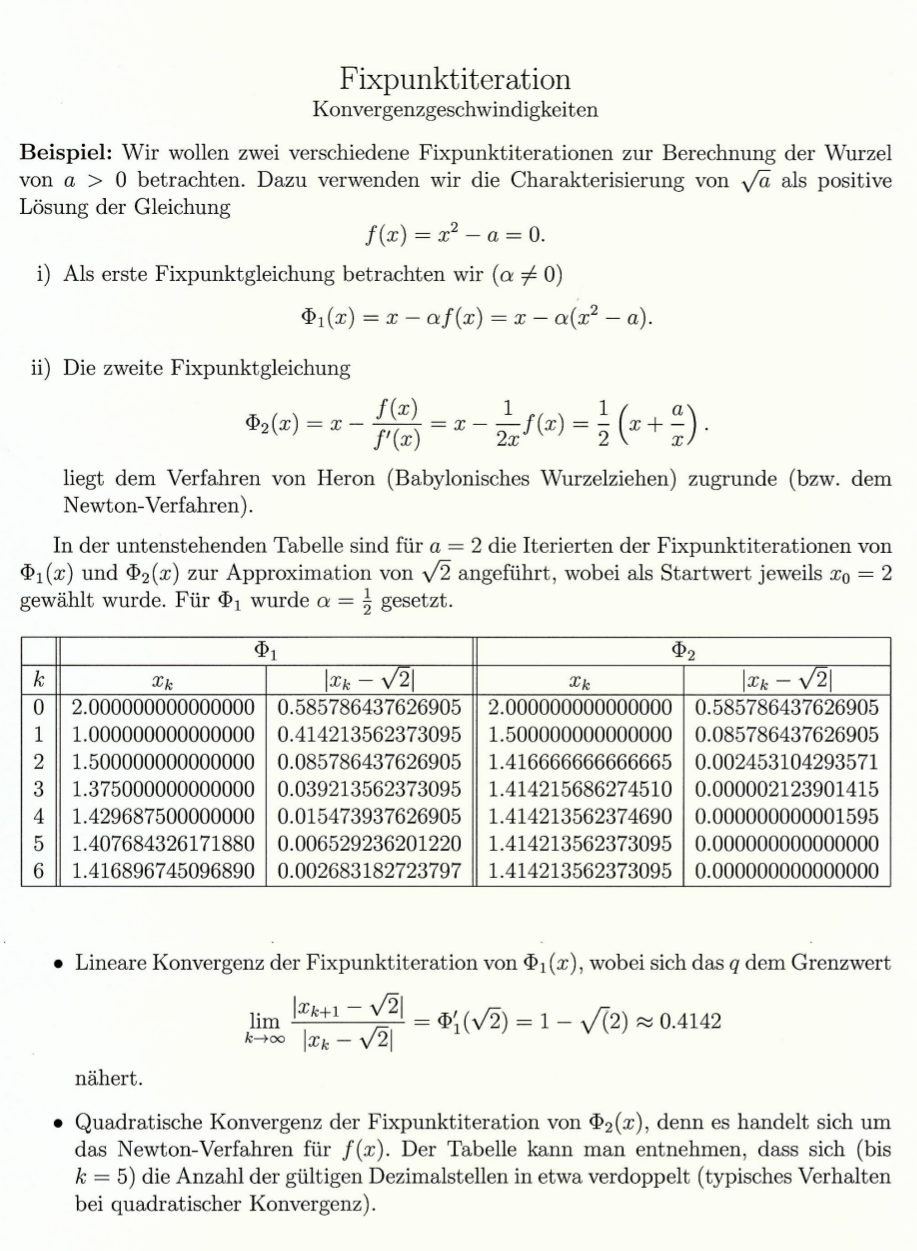
\includegraphics[width=\textwidth]{figures/fixpunktiteration.png}
\end{figure}
\para{Splitting-Verfahren für $Ax = b$}
Sei $A$ regulär. $A = M - N$ ($M$ regulär)
\begin{align*}
  Ax = b \Leftrightarrow Mx = nx + b \Leftrightarrow x = M^{-1} (Nx+b) = \underbrace{M^{-1}Nx + M^{-1}b}_{=: \Phi(x)}
\end{align*}
Fixpunktiteration: $x^{k+1} = \Phi(x^k) = M^{-1}Nx^k + M^{-1}b$ (Splittingverfahren)\\
\satz Sei $B \in \mathbb{K}^{n \times n}$ mit $\norm{B} < 1$. Sei $a \in \mathbb{K}^n$. Dann gilt:
\begin{enumerate}[a)]
  \item Die Fixpunktgleichung $x = Bx + a$ besitzt einen eundeutigen Fixpunkt $x$.
  \item $x^{k+1} := Bx^k + a$ konvergiert gegen $x$ für jedes $x^0$.
\end{enumerate}
\beweis $\Phi(x) := Bx + a$ z.z. ist: $\Phi$ ist Kontraktion.\\
\begin{align*}
  \norm{\Phi(y) - \Phi(z)} = \norm{By + a - Bz - a} = \norm{B(y - z)} \leq \underbrace{\norm{B}}_{= q < 1} \norm{y - z}
\end{align*}
Konsequenz: Das Splitting-Verfahren konvergiert gegen $x = A^{-1}b$, wenn $\norm{M^{-1}N} < 1$. (Es
lässt sich zeigen, dass das Splitting-Verfahren genau dann konvergiert, wenn die Beträge der Eigenwerte
von $M^{-1}N < 1$ sind.)
%subsubsubsubsection 5.4.1.1.1
\para{$\quad$Jacobi-Verfahren}
\begin{align*}
  A = \underbrace{D}_{=: M} + \underbrace{L + R}_{=: -N} \qquad D = \mat{a_{11} & & \\ & \ddots & \\ & & a_{nn}} \qquad
  L = \begin{pmatrix}
    0      &        &        & 0 \\
    a_{21} & \ddots &        &   \\
    \vdots & \ddots & \ddots &   \\
    a_{n1} & \ldots & a_{n,n-1} & 0
  \end{pmatrix}
\end{align*}
\begin{align*}
  Ax = b \Leftrightarrow Dx = -(L+R)x + b \Leftrightarrow x = -D^{-1} \left[ (L+R) - b \right]
\end{align*}
\satz Sei $A$ strikt zeilen- oder strikt spaltendiagonaldominant, dann konvergiert das Jacobi-Verfahren.\\
Strikt zeilendiagonaldominant: $\abs{a_{ii}} > \sum^{n}_{j=1,j \neq i} \abs{a_{ij}} \text{ für } i=1,\ldots,n$
\begin{align*}
  q = \underset{i}{\max} \frac{\sum^{n}_{j=1,j \neq i} \abs{a_{ij}}}{\abs{a_{ii}}}
\end{align*}
%subsubsubsubsection 5.4.1.1.1
\para{$\quad$Gauß-Seidel-Verfahren}
$A = L + D + R$ wie oben
\begin{align*}
  Ax = b \Leftrightarrow (D + L)x = -Rx + b \Leftrightarrow x = - \underbrace{(D+L)^{-1}}_{\text{Vorwärtseinsetzen}}[Rx - b]
\end{align*}
\satz Das Gauß-Seidel-Verfahren konvergiert wenn $A$ s.p.d. ist oder strikt zeilen- bzw. spaltendiagonaldominant ist.\\
\beweis Numerik-Lehrbuch
%subsubsubsection 5.4.1.2
\para{Krylov-Raum-Verfahren}
Schreibweise: $\inner{.}{.}_ = (.,.)$\\
Meistverwendete iterative Verfahren\\
Idee: Wähle Folge von affinen Unterräumen $U_1 \subset U_2 \subset U_3 \ldots$ und suche 
Approximation $x^k \in U^k$ so dass $x^k$ gewisse Eigenschaft (z.B. BA, minimales Residuum, \ldots) erfüllt.\\
\definition Sei $A \in \mathbb{K}^{n \times m}$ und $v \in \mathbb{K}^n$. Für $l \in \mathbb{N}$ bezeichnet man
\begin{align*}
  \mathcal{K}_l(A,v) := \mathrm{span} \left \{ v, Av, A^2v, \ldots, A^{l-1}v \right \}
\end{align*}
als Krylov-Räume bezüglich $(A,v)$.\\
\definition Sei $x^0 \in \mathbb{K}^n$ und $U \subset \mathbb{K}^n$ ein Unterraum, dann heißt
\begin{align*}
  x^0 + U := \{x^0 + u: u \in U\}
\end{align*}
affiner Unterraum von $\mathbb{K}^n$.\\
Krylov-Raum-Verfahren: für $Ax = b$ verwenden
\begin{align*}
  & \mathbin{\textcolor{rot}{x^0 + \mathcal{K}(A,r^0)}} \qquad k=1,2,\ldots\\
  & r^0 = Ax^0 - b
\end{align*}
($x^0$ gewählte Startnäherung), als Approximationsräume für $x = A^{-1}b$.\\
\satz: Sei $A \in \mathbb{K}^{n \times n},\,x^0 \in \mathbb{K}^n$ und $b \in \mathbb{K}^n$. Die Lösung von
$Ax = b$ liegt im Raum $x^0 + \mathcal{K}_l(A,r^0)$ für $l \leq n$.
%5.4.1.2.1
\para{$\quad$CG-Verfahren (Conjugate Gradient Method)}
Anwendbar für selbstadjungierte und positiv definite Matrizen.\\
Selbstadjungiert: $A \in \rnxn := A = A^T; \quad A \in \mathbb{C}^{n \times n}\, A = A^*$ jetzt nur $\rnxn$\\
Ansatz: Wähle $x^k$ als BA von $x$ in $x^0 + \mathcal{K}_k(A,r^0)$ bzgl. $\norm{.}_A$.\\
\satz Sei $A$ s.p.D., dann definiert $(x,y)_A := (Ax, y) = y^TAx$ ein Skalarprodukt, das $A$-Skalarprodukt und
$\norm{x}_A := \sqrt{(x,x)_A}$ ist eine Norm.\\
\beweis Einsetzen\\
Konstruktion der BA $x^k \in x^0 + \mathcal{K}_k(A,r^0)$ von $x = A^{-1}b$ bzgl. $\norm{.}_A$.
Der Einfachheit halber: $x^0 = 0$
\begin{align*}
  r^0 &= Ax^0 - b = -b\\
  x^k &\in \mathcal{K}_k(A,r^0) \text{ ist BA von } x \text{ bzgl. } \norm{.}_A\\
  &\Updownarrow\\
  x^k - x &\perp_A \mathcal{K}_k(A,r^0) \tag{*}
\end{align*}
\begin{figure}[htbp]
  \centering
  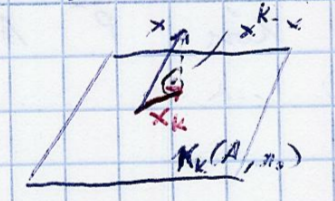
\includegraphics[width=0.3\textwidth]{figures/cg_ba.png}
  \caption{BA Ebene}
\end{figure}
Sei $p^0, p^1,\ldots,p^{k-1}$ $A$-orthogonale Basis von $\mathcal{K}_k(A,r^0)$\\
Ansatz: $x = \sum^{k-1}_{l=0} k_l p^l$
\begin{align*}
  (*) &\Leftrightarrow (x - x^k, p^i)_A = 0 \text{ für } 0,\ldots,k-1\\
      &\Leftrightarrow (x,p^i)_A = (x^k,p^i)_A = (\sum^{k-1}_{l=0} \alpha_l p^l, p^i)_A 
        = \sum^{k-1}_{l=0} \alpha_l(p^l, p^i)_A = \alpha_i(p^i, p^i)_A\\
      &\Rightarrow \alpha_i = \frac{(x,p^i)_A}{(p^i,p^i)_A} \\
      (x,p^i)_A &= (Ax,p^i) = (b,p^i) = -(r^0,p^i)\\
      &\Rightarrow x^k = \sum^{k-1}_{l=0} \alpha_l p^l\\
      r^k &= Ax^k - b = A(x^{k-1} + \alpha_{k-1}p^{k-1}) - b = r_{k-1} + \alpha_{k-1}Ap^{k-1}
\end{align*}
Berechnung von $p^k$: Gram-Schmidt-Verfahren\\
\begin{figure}
  \centering
  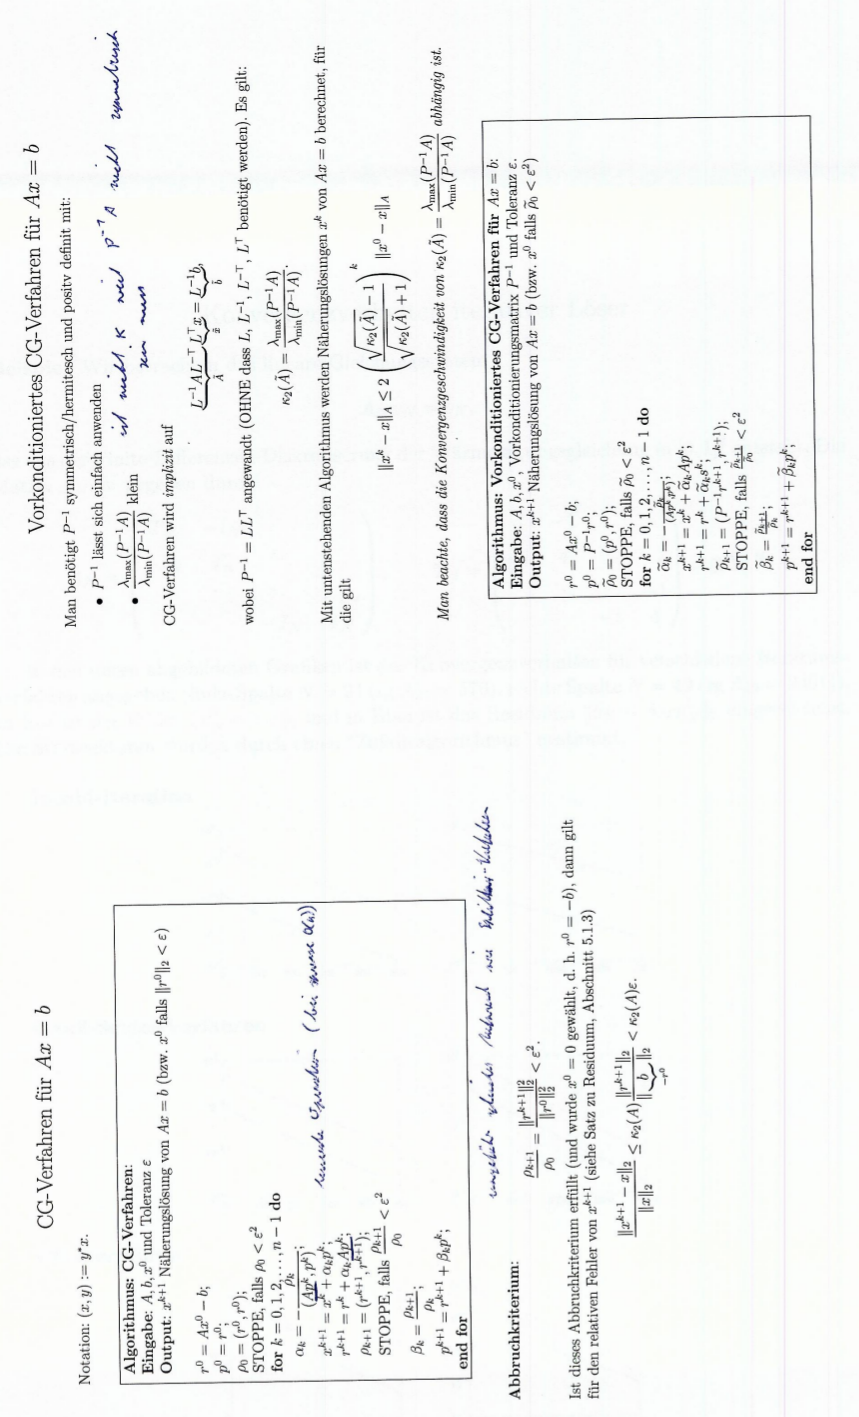
\includegraphics[width=0.9\textwidth]{figures/cg_handout.png}
\end{figure}
\para{$\qquad$Konvergenz des CG-Verfahrens}
Wir wissen bereits:
\begin{itemize}
  \item $\norm{x^{k+1} - x}_A \leq \norm{x^k - x}_A$
  \item $\exists\; l \leq n$, so dass $x^l \in \mathcal{K}_l(A,r^0)$
\end{itemize}
\satz (Fehlerabschätzung des CG-Verfahrens)\\
es gilt ($x^0 \neq x$)
\begin{align*}
  \frac{\norm{x^k - x}_A}{\norm{x^0 - x}_A} < 2 \underbrace{(\frac{\sqrt{\kappa_2(A)} - 1}{\sqrt{\kappa_2(A)}+1} )}_{<1}^k
\end{align*}
\beweis Siehe SAAD
\begin{itemize}
  \item Ist $x^0 = 0$, dann ist obige Abschätzung eine Abschätzung des relativen Fehlers.
  \item Sei $\epsilon > 0$, dann gilt:
  \begin{align*}
    \frac{\norm{x^k - x}_A}{\norm{x^0 - x}_A} < \epsilon
  \end{align*}
  wenn $k \geq \sqrt{\kappa_2(A)} \underbrace{\frac{1}{2} \ln \frac{2}{\epsilon}}$\\
  $\epsilon = 10^{-8} \;\quad\Rightarrow\qquad \;\;9,6$\\
  $\epsilon = 10^{-16} \quad\Rightarrow\qquad 18,8$\\
  $\Rightarrow$ Für $k \geq \sqrt{\kappa_2(A)}19 \Rightarrow \frac{\norm{x^k - x}}{\norm{x^0 - x}} \leq 10^{-16}$
\end{itemize}
\para{$\qquad$Vorkonditioniertes CG-Verfahren}
Allgemeine Idee: Anstelle von $Ax = b$ löse $P^{-1}Ax = P^{-1}b$, wobei
\begin{itemize}
  \item $\kappa(P^{-1}A)$ soll klein sein
  \item $P^{-1}$ muss einfach anwendbar sein
\end{itemize}
Wie bestimmt man $P^{-1}$?\\
Ansatz: Wähle $P^{-1}\approx A^{-1} \Rightarrow P^{-1}A \approx I \Rightarrow \kappa(P^{-1}A) \approx 1$
\begin{itemize}
  \item $P^{-1} = D^{-1}$ (Jacobi-VK)
  \item $P^{-1} = (L + D)^{-1}$ (Gauß-Seidel)
  \item Unvollständige LR-Zerlegung von $A$, d.h. $A = \tilde{L}\tilde{R} + F, \quad P = \tilde{L}\tilde{R}$ $A$ dünnbesetzt:
    \begin{itemize}
      \item $\tilde{r}_{ij} = \tilde{l}_{ij} = 0$ falls $a_{ij} = 0$
      \item $(\tilde{L}\tilde{R})_{ij} = a_{ij}$
      \item $\tilde{l}_{ii} = 1$
    \end{itemize}
    (Zerlegung kann auch nicht existieren, dann nicht anwendbar)\\
    \matlab{ilu}
  \item Unvollständige Cholesky-Zerlegung \matlab{cholinc}
  \item VK-Strategien, die Eigenschaften des zugrundeliegenden Problems ausnutzen
\end{itemize}

\subsubsection{Weitere Krylov-Raum Löser}
Literatur: SAAD, frei online verfügbar
\begin{itemize}
  \item GMRES (Generalized Minimal Residual Method)
    \begin{itemize}
      \item anwendbar für beliebige Matrizen
      \item Verfahren minimiert das Residuum in $x^0 + \mathcal{K}_k(A,r^0)$
      \item Nachteil gegenüber CG: gesamte $\mathcal{K}_k(A,r^0)$ muss gespeichert werden. Daher: Restarts
      \item \matlab{gmres}
      \item Konvergenzgeschwindigkeit abhängig von $\kappa_2(A)$
    \end{itemize}
  \item MINRES
    \begin{itemize}
      \item anwendbar auf symmetrische/hermitesche Matrizen (positive Definitheit wird nicht vorausgesetzt)
      \item Spezialversion von GMRES
      \item Vorteil gegenüber GMRES: weniger Speicherbedarf
      \item \matlab{minres}
    \end{itemize}
\end{itemize}
\begin{figure}[htbp]
  \centering
  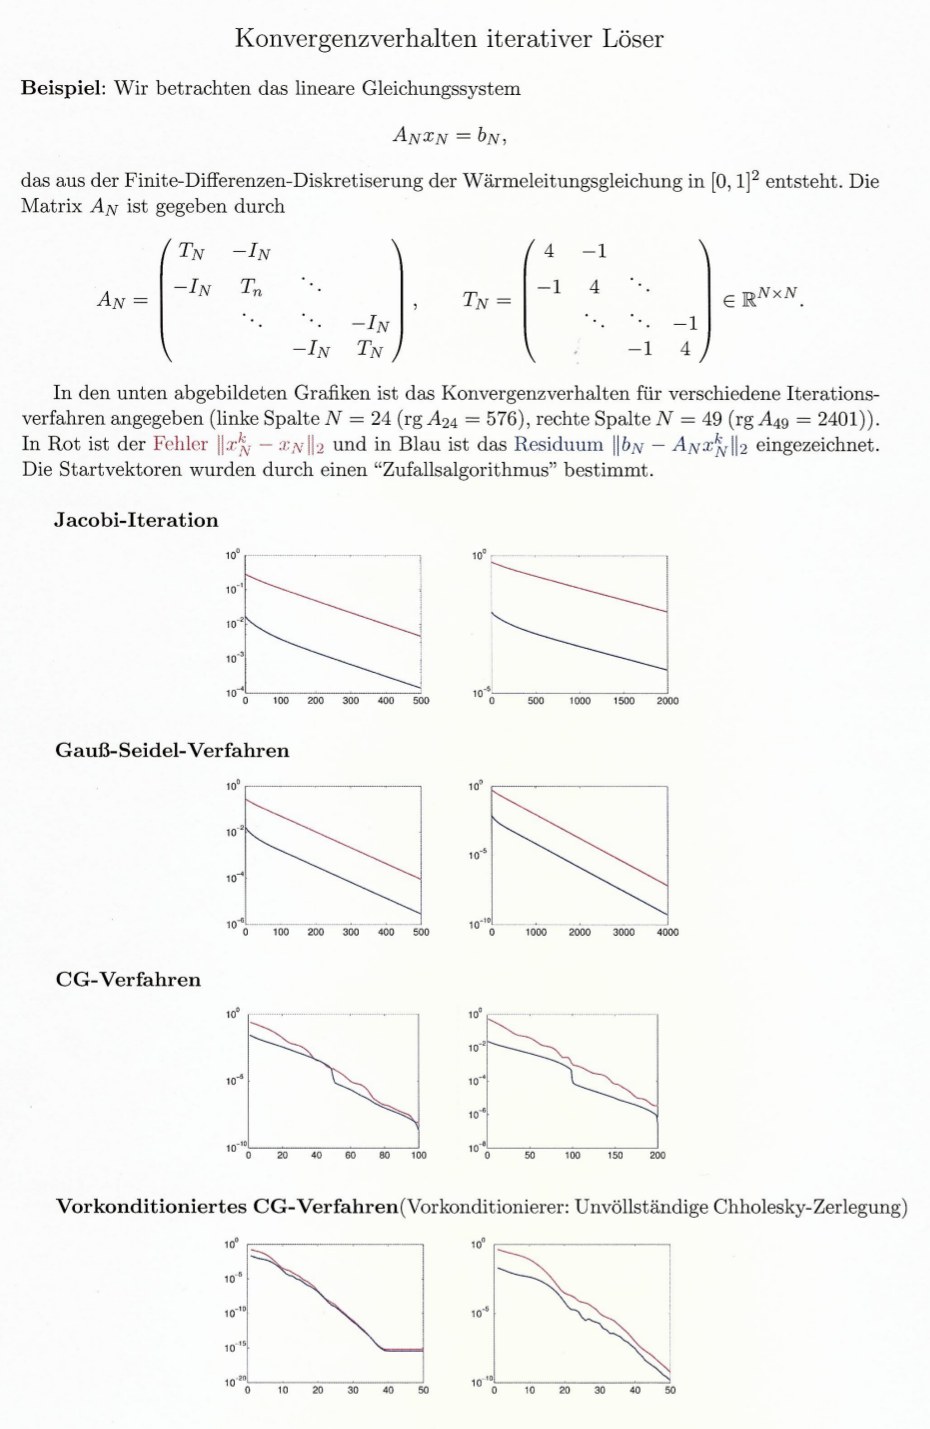
\includegraphics[width=\textwidth]{figures/konv_it_l.png}
\end{figure}













